\documentclass[tikz, border=10pt]{standalone}
\usetikzlibrary{arrows.meta}

\begin{document}
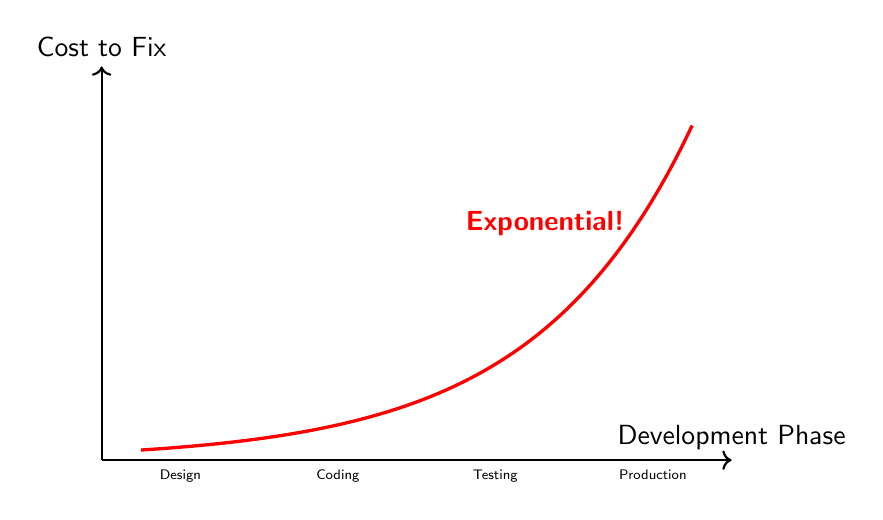
\begin{tikzpicture}[font=\sffamily]

% Axes
\draw[thick, ->] (0,0) -- (8,0) node[above] {Development Phase};
\draw[thick, ->] (0,0) -- (0,5) node[above] {Cost to Fix};

% Curve
\draw[very thick, red, domain=0.5:7.5, samples=100] plot (\x, {0.1*exp(0.5*\x)});

% Labels
\node[below] at (1,0) {\tiny Design};
\node[below] at (3,0) {\tiny Coding};
\node[below] at (5,0) {\tiny Testing};
\node[below] at (7,0) {\tiny Production};

% Callout
\node[red, anchor=west] at (4.5, 3) {\textbf{Exponential!}};

\end{tikzpicture}
\end{document}

